\documentclass[tikz,border=6pt]{standalone}
\usepackage{xcolor}
\begin{document}
% Canonical ch-diagram for 10_1^0,0,1
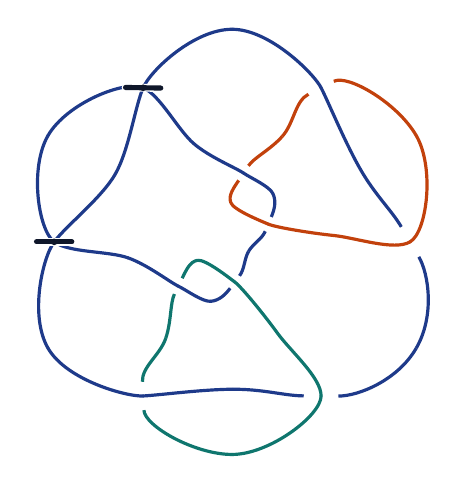
\begin{tikzpicture}[line join=round]
  \definecolor{skcomp0}{RGB}{30,58,138}
  \definecolor{skcomp1}{RGB}{194,65,12}
  \definecolor{skcomp2}{RGB}{15,118,110}
  \definecolor{skmark}{RGB}{15,23,42}
  \draw[skcomp0, line width=1.15pt, line cap=butt] (2.1487,0.1902) .. controls (2.0236,0.4042) and (1.8190,0.5885) .. (1.6252,0.9282);
  \draw[skcomp0, line width=1.15pt, line cap=butt] (2.3711,-0.1902) .. controls (2.4962,-0.4042) and (2.5763,-0.9377) .. (2.3383,-1.3500);
  \draw[skcomp0, line width=1.15pt, line cap=butt] (1.3503,-1.9583) .. controls (1.5982,-1.9597) and (2.1002,-1.7623) .. (2.3383,-1.3500);
  \draw[skcomp1, line width=1.15pt, line cap=butt] (1.2907,2.0391) .. controls (1.4715,2.1314) and (2.1002,1.7623) .. (2.3383,1.3500);
  \draw[skcomp1, line width=1.15pt, line cap=butt] (0.9692,1.8752) .. controls (0.7985,1.7880) and (0.7881,1.5087) .. (0.6360,1.3386);
  \draw[skcomp1, line width=1.15pt, line cap=butt] (0.2075,0.9658) .. controls (0.2774,1.0698) and (0.4838,1.1685) .. (0.6360,1.3386);
  \draw[skcomp1, line width=1.15pt, line cap=butt] (0.0833,0.7809) .. controls (0.0174,0.6826) and (-0.0526,0.5871) .. (-0.0159,0.4959);
  \draw[skcomp0, line width=1.15pt, line cap=butt] (0.4977,0.3163) .. controls (0.5385,0.4129) and (0.5628,0.5159) .. (0.5187,0.6111);
  \draw[skcomp0, line width=1.15pt, line cap=butt] (0.4209,0.1345) .. controls (0.3790,0.0352) and (0.2643,-0.0245) .. (0.2088,-0.1206);
  \draw[skcomp0, line width=1.15pt, line cap=butt] (0.0940,-0.4317) .. controls (0.1590,-0.3458) and (0.1533,-0.2166) .. (0.2088,-0.1206);
  \draw[skcomp0, line width=1.15pt, line cap=butt] (0.9096,-1.9560) .. controls (0.6617,-1.9546) and (0.3999,-1.8695) .. (0.0088,-1.8716);
  \draw[skcomp2, line width=1.15pt, line cap=butt] (-1.1206,-2.1373) .. controls (-1.1101,-2.3401) and (-0.4761,-2.7000) .. (0.0000,-2.7000);
  \draw[skcomp2, line width=1.15pt, line cap=butt] (-1.1393,-1.7770) .. controls (-1.1492,-1.5855) and (-0.9125,-1.4369) .. (-0.8413,-1.2201);
  \draw[skcomp2, line width=1.15pt, line cap=butt] (-0.7326,-0.6626) .. controls (-0.7878,-0.7751) and (-0.7700,-1.0033) .. (-0.8413,-1.2201);
  \draw[skcomp0, line width=1.15pt, line cap=butt] (-0.0251,-0.5891) .. controls (-0.0883,-0.6728) and (-0.1653,-0.7454) .. (-0.2699,-0.7548);
  \draw[skcomp2, line width=1.15pt, line cap=butt] (-0.6346,-0.4626) .. controls (-0.5825,-0.3563) and (-0.5347,-0.2480) .. (-0.4374,-0.2341);
  \draw[skcomp0, line width=1.15pt, line cap=round] (-2.2599,0.0000) .. controls (-2.1105,0.2026) and (-1.6592,0.5571) .. (-1.4856,0.8577);
  \draw[skcomp0, line width=1.15pt, line cap=round] (-1.1300,1.9571) .. controls (-1.2307,1.7264) and (-1.3120,1.1583) .. (-1.4856,0.8577);
  \draw[skcomp0, line width=1.15pt, line cap=round] (-2.2599,0.0000) .. controls (-2.4625,0.1494) and (-2.5763,0.9377) .. (-2.3383,1.3500);
  \draw[skcomp0, line width=1.15pt, line cap=round] (-1.1300,1.9571) .. controls (-1.3607,2.0579) and (-2.1002,1.7623) .. (-2.3383,1.3500);
  \draw[skcomp0, line width=1.15pt, line cap=round] (-2.2599,0.0000) .. controls (-2.4093,-0.2026) and (-2.5763,-0.9377) .. (-2.3383,-1.3500);
  \draw[skcomp0, line width=1.15pt, line cap=round] (-1.1300,-1.9571) .. controls (-1.3327,-1.9677) and (-2.1002,-1.7623) .. (-2.3383,-1.3500);
  \draw[skcomp0, line width=1.15pt, line cap=round] (-2.2599,0.0000) .. controls (-2.0686,-0.1411) and (-1.5700,-0.1141) .. (-1.3210,-0.2032);
  \draw[skcomp0, line width=1.15pt, line cap=round] (-0.6836,-0.5626) .. controls (-0.7961,-0.5074) and (-1.0721,-0.2924) .. (-1.3210,-0.2032);
  \draw[skcomp0, line width=1.15pt, line cap=round] (-1.1300,1.9571) .. controls (-0.9121,1.8620) and (-0.6862,1.4167) .. (-0.4845,1.2456);
  \draw[skcomp0, line width=1.15pt, line cap=round] (0.1454,0.8733) .. controls (0.0414,0.9432) and (-0.2828,1.0746) .. (-0.4845,1.2456);
  \draw[skcomp0, line width=1.15pt, line cap=round] (-1.1300,1.9571) .. controls (-1.0292,2.1879) and (-0.4761,2.7000) .. (0.0000,2.7000);
  \draw[skcomp0, line width=1.15pt, line cap=round] (1.1300,1.9571) .. controls (1.0377,2.1380) and (0.4761,2.7000) .. (0.0000,2.7000);
  \draw[skcomp0, line width=1.15pt, line cap=round] (1.1300,1.9571) .. controls (1.2222,1.7763) and (1.4314,1.2679) .. (1.6252,0.9282);
  \draw[skcomp1, line width=1.15pt, line cap=round] (2.2599,0.0000) .. controls (2.0578,-0.1181) and (1.5733,0.0520) .. (1.2915,0.0809);
  \draw[skcomp1, line width=1.15pt, line cap=round] (0.4593,0.2254) .. controls (0.5616,0.1822) and (1.0097,0.1099) .. (1.2915,0.0809);
  \draw[skcomp1, line width=1.15pt, line cap=round] (2.2599,0.0000) .. controls (2.4739,0.1251) and (2.5763,0.9377) .. (2.3383,1.3500);
  \draw[skcomp1, line width=1.15pt, line cap=round] (0.4593,0.2254) .. controls (0.3570,0.2686) and (0.0207,0.4046) .. (-0.0159,0.4959);
  \draw[skcomp0, line width=1.15pt, line cap=round] (0.1454,0.8733) .. controls (0.2495,0.8035) and (0.4746,0.7064) .. (0.5187,0.6111);
  \draw[skcomp2, line width=1.15pt, line cap=round] (1.1300,-1.9571) .. controls (1.1312,-1.7230) and (0.7416,-1.3885) .. (0.5757,-1.1589);
  \draw[skcomp2, line width=1.15pt, line cap=round] (0.0345,-0.5104) .. controls (0.1230,-0.5774) and (0.4097,-0.9293) .. (0.5757,-1.1589);
  \draw[skcomp0, line width=1.15pt, line cap=round] (-1.1300,-1.9571) .. controls (-0.9272,-1.9466) and (-0.3824,-1.8736) .. (0.0088,-1.8716);
  \draw[skcomp2, line width=1.15pt, line cap=round] (1.1300,-1.9571) .. controls (1.1286,-2.2050) and (0.4761,-2.7000) .. (0.0000,-2.7000);
  \draw[skcomp0, line width=1.15pt, line cap=round] (-0.6836,-0.5626) .. controls (-0.5711,-0.6178) and (-0.3745,-0.7642) .. (-0.2699,-0.7548);
  \draw[skcomp2, line width=1.15pt, line cap=round] (0.0345,-0.5104) .. controls (-0.0541,-0.4435) and (-0.3401,-0.2203) .. (-0.4374,-0.2341);
  \draw[white, line width=2.8pt, line cap=round] (-2.0361,0.0000) -- (-2.4837,0.0000);
  \draw[skmark, line width=1.85pt, line cap=round] (-2.0361,0.0000) -- (-2.4837,0.0000);
  \fill[skmark] (-2.2599,0.0000) circle (1.2pt);
  \draw[white, line width=2.8pt, line cap=round] (-1.3537,1.9610) -- (-0.9062,1.9533);
  \draw[skmark, line width=1.85pt, line cap=round] (-1.3537,1.9610) -- (-0.9062,1.9533);
  \fill[skmark] (-1.1300,1.9571) circle (1.2pt);
\end{tikzpicture}
\end{document}
